\documentclass[german,10pt]{beamer}
\usepackage{tcolorbox}
\usepackage{bm}
\usepackage{graphicx} \graphicspath{ {./figs/} }
%% Integer set
\newcommand{\field}[1]{\mathbb{#1}}
\newcommand{\Rset}{\field{R}}
\newcommand{\Zset}{\field{Z}}
\newcommand{\Qset}{\field{Q}}
\newcommand{\Nset}{\field{N}}

\usetheme{Madrid}
\usepackage{tikz}
\usetikzlibrary{calc}
\usepackage{xcolor}
% Beamer specific settings

% Other styles can be used instead of Boadilla, e.g., to add an index column.
\mode<presentation>
{
  \usetheme{Boadilla} % Without index, with footer
}

\title{CE 401/5501: Good-old-fashioned AI}
% \subtitle{More Essential toward AGI - amid GenAI Hypes}
\author[]{Professor ZhiQiang Chen}
\date{}
\institute[UMKC]
{
  School of Science and Engineering \\
  University of Missouri-Kansas City
}

% This command makes the logo appear at the right side which does not fit
% the UGent style. A solution is found further below.
% \logo{\includegraphics[scale=0.25]{logolabel.jpg}}




% before \begin{document}
\AtBeginSection[]{
  \begin{frame}<beamer>\frametitle{Outline}
    \tableofcontents[currentsection,currentsubsection]
  \end{frame}
  \begin{frame}[plain]
    \centering
    \vfill
    {\usebeamerfont{section title}\insertsectionhead\par}
    \vfill
  \end{frame}
}

\setbeamersize{text margin left=1cm}
\setbeamersize{text margin right=1cm}


\begin{document}

% Title Slide
\frame{\titlepage}

\section{AI by far (covered in this class)}
\begin{frame}{Relations of Classic ML and AI}
    \begin{itemize}
        \item \textbf{Artificial Intelligence (AI):} Simulates human intelligence and behaviors, enabling decision-making and reasoning.
        \item \textbf{Machine Learning (ML):} A subfield of AI focused on creating models that generalize from data to make predictions.
    \end{itemize}
    \begin{tcolorbox}[colframe=blue!75!black, colback=blue!10]
        \textbf{Key Insight:} AI encompasses ML, which primarily relies on inductive reasoning to generalize patterns.
    \end{tcolorbox}
        \begin{figure}[ht]
        \centering     
\includegraphics[width=0.4\textwidth]{./figs/Figure0103.png}
        \caption{AI and ML relationships.}
        \label{lec_01_fig03}
    \end{figure}
\end{frame}

% Slide: Summary of Classic ML Methods
\begin{frame}{Classic ML Methods that we covered:}
  \begin{itemize}
    \item \textbf{Logistic Regression}: Linear classification; outputs probabilities via the sigmoid function.
    \item \textbf{Perceptron and MLPs}: Single-/multi-layer neural networks; learns via margin-based updates; classification and regression. 
    \item \textbf{Support Vector Machine}: Max-margin classifier with kernelized decision boundaries; classification and regression.
    \item \textbf{Bayesian  Classifiers}: Generative probabilistic model assuming independent features (e.g., Naive Bayes).
    \item \textbf{k-Means Clustering}: Unsupervised grouping into \(k\) clusters by minimizing within-cluster variance.
    \item \textbf{Deep Neural Networks}: Multi-layer, data-driven feature extraction and representation learning.
  \end{itemize}
  \begin{alertblock} { All are data-driven models, which are }
  \begin{itemize}
      \item  Either \textit{connectionist} - most are neural-network-like models (MLPs, CNNs, RNNs, etc.)
      \item  Or \textit{statistical} - most focus on learning from data with statistical/probabilistic modeling (e.g., SVMs, Naive Bayes, EM algorithm)
  \end{itemize}
    
  \end{alertblock}
\end{frame}

\section{Motivation for GOFAI}

% Slide: Human Reasoning – Observations vs. Rules
\begin{frame}{Human Reasoning: Observations vs. Rules}
\begin{block}{Key Question}
    Do humans reason based solely on observations (data)?
\end{block}
\begin{itemize}
    \item Infants rely on sensory experience, but quickly incorporate language and instruction.
    \item We acquire formal rules through grammar, mathematics, and logic.
\end{itemize}
\begin{block}{Early AI Motivation}
    Pioneers such as Alan Turing (1950), John McCarthy (1955), Marvin Minsky (1956), and Herbert Simon \& Allen Newell (1956) argued for symbolic systems to capture this rule-based aspect of human thought.
\end{block}
\begin{columns}[t]
    \column{0.48\textwidth}
      \centering
      
\includegraphics[width=\textwidth]{./figs/Turning.png}
      \\*\small Alan Turing, “Computing Machinery and Intelligence” (1950)
    \column{0.3\textwidth}
      \centering
      
\includegraphics[width=\textwidth]{./figs/McCarthy.png}
      \\*\small John McCarthy, “Programs with Common Sense” (1958)
  \end{columns}
\end{frame}

% Slide 2: Defining GOFAI
\begin{frame}{Defining GOFAI: Basic Features}
  \begin{itemize}
    \item \textbf{Symbolic representation}: Use of discrete symbols to model entities and relationships in a human-readable form. 
      \begin{itemize}
        \item Example: Representing facts as predicates, e.g., \textit{Parent(John, Mary)} denotes that John is a parent of Mary.
      \end{itemize}
    \item \textbf{Rule-based reasoning}: Application of explicit IF–THEN rules to infer new knowledge.
      \begin{itemize}
        \item Example: \emph{IF} \texttt{Parent(x,y)} \emph{AND} \texttt{Parent(y,z)} \emph{THEN} \texttt{Grandparent(x,z)}.
      \end{itemize}
\end{itemize}
\begin{alertblock}{Contrast with data-driven ML}
    \begin{itemize}
        \item Connectionist (e.g., neural networks) and statistical (e.g., probabilistic models) methods learn patterns from data 
        \item Symbolic AI (or Rule-based AI) uses explicit symbols to represent knowledge and rules (logic-based or procedural) to manipulate those symbols
    \end{itemize}
\end{alertblock}
\end{frame}

\section{GOFAI Basics}
%% Slide 3: Historical Milestones
\begin{frame}{Historical Milestones - 1}
  \begin{itemize}
    \item \textbf{\textcolor{blue}{Logic Theorist} (Newell \& Simon, 1956)}
    \item \textbf{\textcolor{blue}{General Problem Solver} (Newell \& Simon, 1957)}
    \item \textbf{\textcolor{blue}{SHRDLU} (Winograd, 1970)}
    \item \textbf{\textcolor{red}{AI Winter I} (mid-1970s): Funding cuts and skepticism after early optimism}
    \item \textbf{\textcolor{blue}{Expert Systems Boom (1980s)}: Industry adoption (e.g., XCON, DENDRAL, PROSPECTOR)}
    \item \textbf{\textcolor{red}{AI Winter II} (late-1980s–early-1990s): Collapse of the expert-systems market}
  \end{itemize}
\end{frame}

\begin{frame}{Historical Milestones - 2}
  \begin{itemize}
    \item \textbf{Resurgence of Machine Learning (late-1980s–2000s):}
      \begin{itemize}
        \item Neural networks revival (Rumelhart et al., 1986); Support Vector Machines (Cortes \& Vapnik, 1995); Graphical Models: Bayesian networks, Markov random fields (1990s)
      \end{itemize}
    \item \textbf{\textcolor{blue}{Semantic Web \& Knowledge Graphs (2000s)}:} RDF/OWL, SPARQL, Linked Data
    \item \textbf{Deep Learning Revolution (2010s):} Convolutional networks, transformers
    \item \textbf{Generative AI (2020s–present):} Large-scale language models, diffusion models
    \item \textbf{\textcolor{green}{Neurosymbolic AI (2010s–present):}} Logic Tensor Networks, DeepProbLog, differentiable ILP
  \end{itemize}
\end{frame}


\begin{frame}{Historical Milestones}
  \centering
  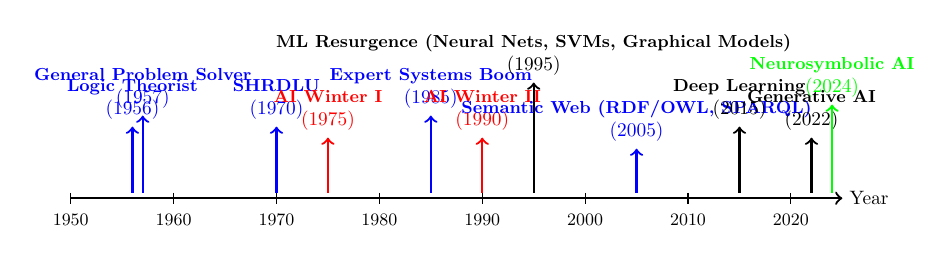
\begin{tikzpicture}[scale=0.7, transform shape]
    % (Ensure you have \usetikzlibrary{calc} in your preamble)

    \def\YearStart{1950}
    \def\YearEnd{2025}
    \def\AxisLen{14}

    % Draw axis
    \draw[->, thick] (0,0) -- (\AxisLen,0) node[right]{Year};

    % Ticks every decade
    \foreach \y in {1950,1960,1970,1980,1990,2000,2010,2020} {
      \pgfmathsetmacro{\x}{(\y-\YearStart)/(\YearEnd-\YearStart)*\AxisLen}
      \draw (\x,0.1) -- (\x,-0.1) node[below=2pt]{\small \y};
    }

    % Milestones: event/year/vertical offset/color
    \foreach \event/\year/\offset/\col in {
      {Logic Theorist}/1956/1.2/blue,
      {General Problem Solver}/1957/1.4/blue,
      {SHRDLU}/1970/1.2/blue,
      {AI Winter I}/1975/1.0/red,
      {Expert Systems Boom}/1985/1.4/blue,
      {AI Winter II}/1990/1.0/red,
      {ML Resurgence (Neural Nets, SVMs, Graphical Models)}/1995/2.0/black,
      {Semantic Web (RDF/OWL, SPARQL)}/2005/0.8/blue,
      {Deep Learning}/2015/1.2/black,
      {Generative AI}/2022/1.0/black,
      {Neurosymbolic AI}/2024/1.6/green} 
      {
      \pgfmathsetmacro{\x}{(\year-\YearStart)/(\YearEnd-\YearStart)*\AxisLen}
      \draw[->, thick, color=\col] (\x,0.1) -- ++(0,\offset)
        node[above, align=center]{\small \textbf{\event}\\(\year)};
    }
  \end{tikzpicture}
\end{frame}

\begin{frame}{Symbolic AI Aimed at Development of an Expert System}
  \centering
  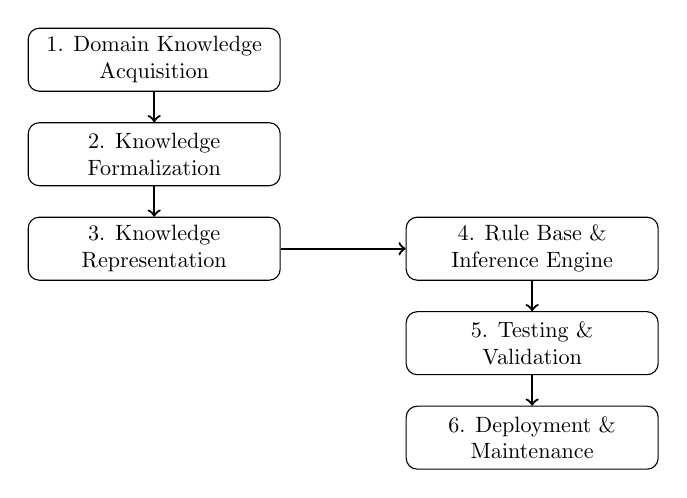
\begin{tikzpicture}[scale=0.8, transform shape]
    % block style
    \tikzstyle{block}=[
      draw,
      rectangle,
      rounded corners,
      minimum width=4cm,
      minimum height=1cm,
      align=center
    ]

    % Left column
    \node[block] (A) at (-3,3) {1. Domain Knowledge\\Acquisition};
    \node[block] (B) at (-3,1.5) {2. Knowledge\\Formalization};
    \node[block] (C) at (-3,0) {3. Knowledge\\Representation};

    % Right column
    \node[block] (D) at (3,0) {4. Rule Base \&\\Inference Engine};
    \node[block] (E) at (3,-1.5) {5. Testing \&\\Validation};
    \node[block] (F) at (3,-3) {6. Deployment \&\\Maintenance};

    % Arrows down left column
    \draw[->, thick] (A.south) -- (B.north);
    \draw[->, thick] (B.south) -- (C.north);

    % Arrow middle cross
    \draw[->, thick] (C.east) -- (D.west);

    % Arrows down right column
    \draw[->, thick] (D.south) -- (E.north);
    \draw[->, thick] (E.south) -- (F.north);
  \end{tikzpicture}
  %\footnotesize
  \begin{alertblock}{Note - two major technical components}
  \begin{itemize}
        \item Knowledge Representation 
        \item Rule Base \& Inference Engine”: predicate logic, unification, and search algorithms are implemented to drive inference.
  \end{itemize}
  \end{alertblock}
\end{frame}



\begin{frame}{Symbolic AI Fundamentals: Knowledge Representation}
  \begin{itemize}
    \item \textbf{Frames \& Objects}  
      – Structured records with named slots, e.g.\ \texttt{Person(name, age, occupation)}.  
      Supports inheritance: \(\texttt{Student}\sqsubseteq\texttt{Person}\).
    \item \textbf{Semantic Networks}  
      – Directed labeled graphs, e.g.\ \(\texttt{Dog}\xrightarrow{\texttt{isA}}\texttt{Mammal}\).  
      Inference via transitive closure on “isA” edges.
    \item \textbf{Ontologies (Description Logics)}  
      – Concept inclusion: \(Dog\sqsubseteq Animal\)  
      – Role restrictions: \(Dog\sqsubseteq \exists hasPart.\,Tail\)  
      – Assertions: \(\texttt{John:Dog}\), \(\texttt{Tail1:Tail}\)
    \item \textbf{Expressivity vs. Efficiency}  
      – \(\mathcal{ALC}\) (PSpace‐decidable) vs.\ \(\mathcal{SROIQ}\)/OWL‑DL (ExpTime)  
      – Higher expressivity $\Rightarrow$ higher reasoning complexity
  \end{itemize}
\end{frame}



\begin{frame}{Symbolic AI Fundamentals: Predicate Logic}
  \begin{itemize}
    \item \textbf{Key idea:} Represent knowledge explicitly using logical statements.
    
    \item \textbf{Clauses (examples):}
    \[
      C_1: P(a) \lor Q(a), \quad C_2: \neg P(a)
    \]
    \begin{itemize}
      \item \(C_1\): "Either \(P(a)\) or \(Q(a)\) (or both) is true."
      \item \(C_2\): "\(P(a)\) is false."
    \end{itemize}
    
    \item \textbf{Resolution rule (general form):}
    \[
      \frac{L \lor \phi,\;\neg L \lor \psi}{\phi \lor \psi}
    \]
    \begin{itemize}
      \item If one clause asserts \(L\) (with some additional terms \(\phi\)) and another asserts its negation \(\neg L\) (with terms \(\psi\)), we infer a new clause combining remaining terms.
    \end{itemize}
    
    \item \textbf{Example of resolution:}
    \[
      \frac{P(a)\lor Q(a),\;\neg P(a)}{Q(a)}
    \]
    \begin{itemize}
      \item Since \(P(a)\) and \(\neg P(a)\) contradict each other, resolution removes them, leaving the new clause \(Q(a)\).
    \end{itemize}
  \end{itemize}
\end{frame}


\begin{frame}{Symbolic AI Fundamentals: Unification}
  \begin{itemize}
    \item \textbf{Purpose:} Match logical statements by identifying compatible substitutions.

    \item \textbf{Definition (Most General Unifier - mgu):}
    \[
      \mathrm{mgu}\bigl(f(x,a),\,f(b,y)\bigr) = \{x\!\mapsto\!b,\;y\!\mapsto\!a\}
    \]
    \begin{itemize}
      \item This identifies the simplest substitutions to make both expressions identical.
    \end{itemize}

    \item \textbf{Interpretation:}  
    Substitute \(x\) with \(b\) and \(y\) with \(a\) to unify:
    \[
      f(x,a)\;\;\to\;\; f(b,a), \quad f(b,y)\;\;\to\;\;f(b,a)
    \]
    \begin{itemize}
      \item After applying these substitutions, both expressions become exactly the same (\(f(b,a)\)), achieving unification.
    \end{itemize}
  \end{itemize}
\end{frame}



\begin{frame}{Symbolic AI Fundamentals: Search \& Production Systems}
  \begin{itemize}
    \item \textbf{Search Algorithms:}
      \begin{itemize}
        \item \textbf{Breadth-First Search (BFS):} Explores nodes by FIFO queue (level-wise exploration).
        \item \textbf{Depth-First Search (DFS):} Explores nodes by LIFO stack (deepest path first).
        \item \textbf{A* Algorithm:}
          \[
            f(n)=g(n)+h(n)
          \]
          Uses admissible heuristic \(h(n)\) for optimal paths.
      \end{itemize}
    \item \textbf{Production Systems (\textit{Rete Algorithm}):}
      \begin{itemize}
        \item Working memory (\(WM\)) and rules (\(R\)):
          \[
            WM_{t+1} = WM_t \cup \{\mathrm{head}(r)\mid r\in R,\;\mathrm{body}(r)\subseteq WM_t\}
          \]
        \item Rete network compiles rules into an efficient shared-test graph.
        \item Complexity of updates reduced significantly to:
          \[
            O(\Delta WM + \Delta R)
          \]
      \end{itemize}
  \end{itemize}
\end{frame}



% \begin{frame}{Implementation of Symbolic AI Algorithms}
%   \begin{itemize}
%     \item \textbf{Logic \& Resolution}  
%       \begin{itemize}
%         \item Unification + backtracking over clauses (e.g., Prolog’s `resolve/2`), recursively deriving new facts.
%       \end{itemize}
%     \item \textbf{Search}  
%       \begin{itemize}
%         \item DFS/BFS: stack or queue frontier.  
%         \item A\*: priority queue keyed by \(f(n)=g(n)+h(n)\) (binary heap for \(O(\log N)\) ops).
%       \end{itemize}
%     \item \textbf{Production Systems}  
%       \begin{itemize}
%         \item Working memory of facts + IF–THEN rules.  
%         \item Rete algorithm: compiles rules into a network, sharing tests, to match thousands of rules efficiently.
%       \end{itemize}
%     \item \textbf{Knowledge Representation}  
%       \begin{itemize}
%         \item Frames → classes/structs with named slots.  
%         \item Semantic nets → adjacency lists or triple stores.  
%         \item Ontologies (RDF/OWL) → stored in graph DBs (e.g., Jena) with built-in reasoners.
%       \end{itemize}
%   \end{itemize}
% \end{frame}

% \begin{frame}{Optimizations \& Languages}
%   \begin{itemize}
%     \item \textbf{Key Optimizations}
%       \begin{itemize}
%         \item \emph{Indexing \& Hashing}: O(1) lookup for facts/rules  
%         \item \emph{Memoization (Tabling)}: cache subgoal results (e.g., XSB Prolog)  
%         \item \emph{Heuristic Pruning}: admissible heuristics in A\*  
%         \item \emph{JIT Compilation}: compile rules to bytecode for native speed  
%         \item \emph{Parallelism}: multi‐threaded/distributed search \& matching  
%       \end{itemize}
%     \item \textbf{Languages \& Frameworks}
%       \begin{itemize}
%         \item \emph{Logic Programming}: Prolog (SWI-Prolog, XSB), Mercury  
%         \item \emph{Lisp Family}: Common Lisp, Clojure  
%         \item \emph{Rule Engines}: CLIPS, Jess, Drools  
%         \item \emph{Triple Stores}: Apache Jena, RDF4J, RDFLib (Python)  
%         \item \emph{General Purpose}: Python, C++, Java (with embedded search/rule libraries)  
%       \end{itemize}
%   \end{itemize}
% \end{frame}

\section{Expert Systems}
% Slide: Expert Systems — Definition & Origins
\begin{frame}{Expert Systems: Definition \& Origins}
  \begin{itemize}
    \item \textbf{What is an Expert System?}  
      A software system that \emph{encodes expert knowledge} in a domain as a set of rules and uses an \emph{inference engine} to draw conclusions.
    \item \textbf{Architecture}: Knowledge base + Inference engine (forward/backward chaining)
    \item \textbf{Early Pioneers}  
      \begin{itemize}
        \item \textbf{DENDRAL} (Feigenbaum \& Buchanan, 1965): chemical‐structure elucidation  
        \item \textbf{MYCIN} (Buchanan \& Shortliffe, 1972): medical diagnosis with certainty factors  
      \end{itemize}
    \item \textbf{Term Coined}:  
      \emph{“Expert System”} popularized mid-1970s at Stanford and Carnegie Mellon AI labs.
  \end{itemize}
\end{frame}

% Slide: Why the Expert Systems Hype?
\begin{frame}{Why the Expert Systems Hype?}
  \begin{itemize}
    \item \textbf{Promise of Automation}  
      Capture scarce human expertise (medicine, engineering design, finance) in software.
    \item \textbf{Business Impact}  
      Consistency, reduced errors, 24/7 availability → large ROI (e.g., XCON saved DEC \$40M/yr).
    \item \textbf{Funding Surge}  
      1980s: Government \& industry poured \$billions into “knowledge-based” initiatives.
    \item \textbf{Limitations Uncovered}  
      \emph{Knowledge‐acquisition bottleneck}, brittleness, difficulty scaling to new domains.
  \end{itemize}
\end{frame}

% % Slide: Representative Frameworks & Mathematical Foundations
% \begin{frame}{Frameworks \& Mathematical Foundations}
%   \begin{itemize}
%     \item \textbf{Production System Complexity}  
%       \[
%         \text{WM}_{t+1} \;=\; \text{WM}_t \;\cup\;\{\,\mathrm{head}(r)\mid r\in R,\;\mathrm{body}(r)\subseteq \text{WM}_t\},
%       \]  
%       naive matching cost \(O(|R|\times|\text{WM}|)\).
%     \item \textbf{Rete Algorithm}  
%       Compiles rules into a network of \(C\) nodes → matching in \(O(\Delta C + \Delta F)\) per update.
%     \item \textbf{Certainty Factors} (MYCIN)  
%       Combine CFs:  
%       \[
%         \mathrm{CF}_{12} \;=\; \mathrm{CF}_1 + \mathrm{CF}_2\,(1-\mathrm{CF}_1).
%       \]
%     \item \textbf{Typical Languages \& Tools}  
%       OPS5, CLIPS, Jess, Drools, Prolog, Lisp — all optimize pattern‐matching, conflict resolution, and inference scheduling.
%   \end{itemize}
% \end{frame}

\begin{frame}{Expert Systems in Engineering Design}
\begin{itemize}
  \item \textbf{Key Historical Applications}:
  \begin{itemize}
    \item XCON (DEC, 1980): Automatic VAX configuration
    \item DENDRAL (Stanford, 1965): Chemical-structure elucidation
    \item PROSPECTOR (Stanford, 1978): Geologic exploration guidance
    \item ICAD (MIT, 1988): Parametric CAD for mechanical parts
    \item CADEX/KEE (Intel, early 1980s): Engineering advisory shells
  \end{itemize}
  \item Benefits: Codified best practices, reduced design time
  % \item Lessons: Knowledge-acquisition bottleneck, maintenance challenges
\end{itemize}
\end{frame}

\begin{frame}{Expert Systems in Structural Design: \href{https://doi.org/10.1016/0010-4485(85)90289-1}{\textit{HI-RISE}, CMU 1985 - 1987} }
  \begin{itemize}
    % \item \textbf{Source}: CMU Tech Report No. 14642114 (July 2006) — “Knowledge‐Based Expert Systems in Structural Design” :contentReference[oaicite:0]{index=0}
    \item \textbf{Recognized Challenge}:  
      \textit{Many structural design problems are ill‐structured and resist purely algorithmic solutions}
    \item \textbf{Approach}:  
      \begin{itemize}
        \item Encode engineering heuristics and design rules in a symbolic knowledge base  
        \item Inference engine performs forward/backward chaining to derive design decisions  
        \item Integrate case‐based reasoning to retrieve and adapt previous design examples
      \end{itemize}
    % \item \textbf{Key Contributions}:  
    %   \begin{itemize}
    %     \item Demonstrates rule‐based support for concept‐level member sizing and load analysis  
    %     \item Shows improved design consistency, reduced iteration cycles  
    %     % \item Lays groundwork for CAD‐integrated design assistants
    %   \end{itemize}
    \item \textbf{Impact}:  
      \begin{itemize}
        \item Pioneer in applying symbolic AI to civil‐engineering design automation  
        \item Influenced later systems combining CAD, expert‐system shells, and knowledge graphs
      \end{itemize}
  \end{itemize}
\end{frame}


\begin{frame}{Expert Systems in Structural Design: \href{https://doi.org/10.1016/0010-4485(85)90289-1}{\textit{HI-RISE}, CMU 1985 - 1987} }
\begin{figure}
    \centering
    
\includegraphics[width=0.5\linewidth]{figs/Maher1985.png}
    \caption{Realized workflow - \textit{HI-RISE} at CMU (courtesy of Maher, 1987)}
    \label{fig:enter-label}
\end{figure}

\end{frame}

% Slide 7: Limitations & Criticisms
\begin{frame}{Limitations \& Criticisms}
\begin{itemize}
  \item Brittleness \& the frame problem
  \item Knowledge engineering bottleneck
  \item Scalability and maintenance issues
\end{itemize}
\end{frame}
\section{GOFAI: Good for AGI?}

% Slide: Modern Generative AI vs. GOFAI – Strengths & Limitations
\begin{frame}{Modern Generative AI vs. GOFAI}
  \begin{columns}[t]
    \column{0.48\textwidth}
      \textbf{Generative AI (Connectionist)}  
      \begin{itemize}
        \item \textbf{Strengths:}
          \begin{itemize}
            \item Learns rich representations from large‑scale data  
            \item Excels at pattern completion, language generation, vision tasks  
            \item Robust to noise and distributional variation
          \end{itemize}
        \item \textbf{Limitations:}
          \begin{itemize}
            \item Opaque “black‑box” reasoning, poor explainability  
            \item Requires massive annotated datasets  
            \item Struggles with precise constraints and logical consistency
          \end{itemize}
      \end{itemize}

    \column{0.48\textwidth}
      \textbf{GOFAI (Symbolic)}  
      \begin{itemize}
        \item \textbf{Strengths:}
          \begin{itemize}
            \item Explicit, human‐readable rules and logic  
            \item Strong guarantees on constraint satisfaction and inference  
            \item Easily auditable and explainable decision paths
          \end{itemize}
        \item \textbf{Limitations:}
          \begin{itemize}
            \item Knowledge‐acquisition bottleneck (expert elicitation)  
            \item Brittleness: poor generalization outside coded rules  
            \item Scalability issues as rule base grows
          \end{itemize}
      \end{itemize}
  \end{columns}
\end{frame}

% Slide: Neuro‑Symbolic & Hybrid AI Efforts
\begin{frame}{Neuro‑Symbolic \& Hybrid AI Efforts}
  \begin{itemize}
    \item \textbf{Neuro‑Symbolic Frameworks}
      \begin{itemize}
        \item \emph{LogicTensorNetworks}: integrate fuzzy logical constraints into neural training \cite{Garcez2009}.
        \item \emph{DeepProbLog}: neural predicates within Prolog for perception‑driven reasoning.
        \item \emph{Neuro‑Symbolic Transformers}: embed logical modules in transformer layers \cite{Xu2023}.
      \end{itemize}
    \item \textbf{Toolkits \& APIs}
      \begin{itemize}
        \item LangChain / LlamaIndex: hook LLMs to external symbolic engines (Prolog, OWL reasoners).
        \item Pyke, DeepKE: Python libraries for rule‑based inference alongside ML pipelines.
      \end{itemize}
    \item \textbf{Applications}
      \begin{itemize}
        \item Knowledge‑guided code synthesis, program verification  
        \item Constrained generative design in CAD and architecture  
        \item Explainable clinical decision support combining EHR data with medical ontologies
      \end{itemize}
  \end{itemize}
\end{frame}

% Slide: Future Directions & Vision toward AGI/SMI
\begin{frame}{Future Directions \& Vision toward AGI/AMI}
  \begin{itemize}
    \item \textbf{Scalable Neuro‑Symbolic Architectures}  
      \begin{itemize}
        \item Modular “cognitive stacks” combining perception, memory, and reasoning.  
        \item Federated rule repositories with learned embeddings.
      \end{itemize}
    \item \textbf{Trustworthy Advanced Machine Intelligence (AMI) }  
      \begin{itemize}
        \item Built‐in audit logs of symbolic trace alongside statistical confidence.  
        \item Self‑explanation and on‑the‑fly rule refinement.
      \end{itemize}
    \item \textbf{Standardization \& Benchmarks}  
      \begin{itemize}
        \item Unified neuro‑symbolic evaluation suites (CLEVRX, LogicalQA).  
        \item Community‐driven frameworks for interface consistency.
      \end{itemize}
    \item \textbf{Long‑Term Vision}  
      \begin{itemize}
        \item AI systems with human‑level adaptability, commonsense, and verifiable safety.  
        \item AGI/AMI as collaborative partners in science, engineering, and creativity.
      \end{itemize}
  \end{itemize}
\end{frame}

\section{Conclusions}
\begin{frame}{Conclusions }
  \begin{itemize}
    \item GOFAI methods offer transparent, rule-based reasoning with strong explainability - broadly termed symbolic AI.
    \item Expert systems showcased earlier efforts toward domain automation but faced scalability and maintenance challenges.
    \item Neuro-symbolic techniques combine symbolic constraints and statistical learning for robust AI.
    \item FINALLY: \textcolor{red}{\textit{Scalable neuro-symbolic AI represents a promising pathway toward achieving AGI (Artificial General Intelligence) or AMI (Autonomous Machine Intelligence)}.}
  \end{itemize}
\end{frame}



% Slide 13: References
\begin{frame}{References}

\begin{thebibliography}{10}
 {\tiny
\beamertemplatebookbibitems
\bibitem{RussellNorvig}
  S.~Russell and P.~Norvig,
  \emph{Artificial Intelligence: A Modern Approach}, 4th~ed., 2020.
\bibitem{NewellSimon}
  A.~Newell and H.~A.~Simon,
  "Computer Science as Empirical Inquiry: Symbols and Search," 1976.
\bibitem{MuggletonDeRaedt}
  S.~Muggleton and L.~De~Raedt,
  "Inductive Logic Programming," New Generation Computing, 1994.
\bibitem{GarcezEtAl}
  A.~d'Avila Garcez, L.~De~Raedt, and K.~K"ung,
  \emph{Neural-Symbolic Cognitive Reasoning}, 2009.
\bibitem{Maher1985} 
    M.~Maher. \emph{HI-RISE and beyond: directions for expert systems in design,} Computer-aided design 17, no. 9 (1985): 420-427.
    \bibitem{Garcez2009}
      A.~d'Avila Garcez, L.~De~Raedt, and K.~K\"ung. \emph{Neural‐Symbolic Cognitive Reasoning}. IOS Press, 2009.
    \bibitem{Clark2020}
      P.~Clark et al. “Transformers as Soft Reasoners over Language,” \emph{Findings of the Association for Computational Linguistics}, 2020.
    \bibitem{Xu2023}
      M.~Xu and M.~Lewis. “Neuro‐Symbolic Transformers for Structured Reasoning,” \emph{Journal of AI Research}, 2023.
    \bibitem{Marcus2022}
      G.~Marcus and E.~Davis. “Neuro‐Symbolic AI: The State of the Art,” \emph{Communications of the ACM}, 2022.
    \bibitem{IEEE7010}
      IEEE Standards Association. \emph{Recommended Practice for Addressing Ethical Concerns in Building Autonomous Systems (IEEE P7010)}, 2021.
      }
\end{thebibliography}

\end{frame}

\end{document}
